\ifx\wholebook\relax\else
\input{../Common.tex}
\input{../macroes.tex}
\begin{document}
\fi

\project
\chapter{Parametric L-Systems}\label{ch:parametric}

\begin{chapterfigure}
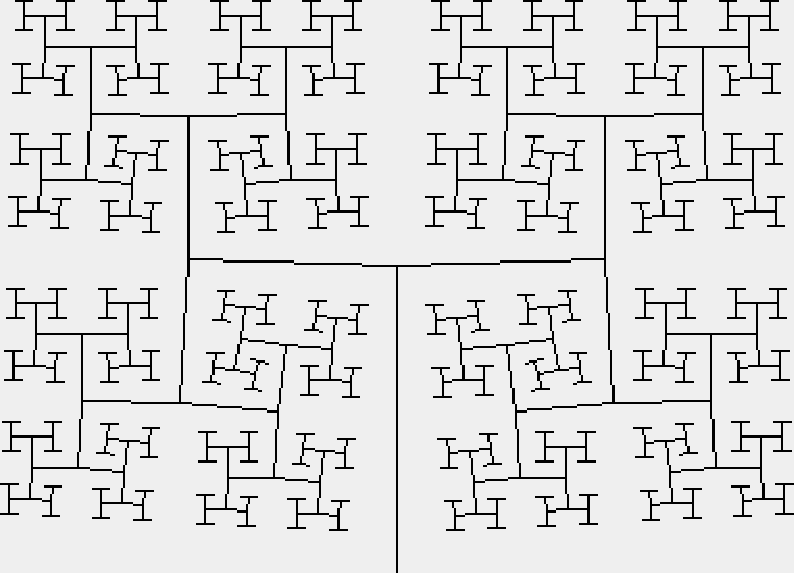
\includegraphics[width=12cm]{Growing}
\end{chapterfigure}


One of the limits of L-Systems that we have seen so far is that we
cannot manipulate any parameters like angle or length to be drawn. The
only way we have was to use rules to rewrite a forward command by
several ones.  Parametric L-Systems propose an answer to such a
problem by providing a way to pass parameters to the rule and
manipulating them.  In this chapter, we propose you to implement this
new kind of L-Systems.  However, we just do not restart from scratch a
new implementation but reuse some of the previous implementation.  Let
us first look at the new aspects of parametric L-Systems.

\section{Parametric L-Systems}\label{sec:param}
The last kind of L-Systems we would like to use is called
\emph{parametric L-System} \emph{(pL-Systems)}. Parametric L-Systems 
allows one to express finer plant growth or fractals. The idea is that
a rule can specify arguments or parameters that are evaluated and
manipulated.

Let us look at two examples: the first parametric L-System produces
the first picture of this chapter, the second one the
Figure~\ref{fig:leaf1}.

\begin{tabbing}
\=aaa\=aaa\=aaa\=aaaaaaaaa\=aaaaaaaaa\=aaaaaaaaa\=aaaaaaaaa\=aaaaaaaaa\=aaaaaaaaa\kill
T \\
\>\>\>\> \emph{Axiom} \>\>\emph{A(0)}\\
\>\>\>\> \emph{Angle} \>\>88 degree\\
\>\>\>\> \emph{Rule}  \>\>\emph{A(d) $\rightarrow$ F(1)[+A(0)][-A(0)]}\\
\>\>\>\> \emph{Rule}  \>\>\emph{F(d) $\rightarrow$ F(d * 1.456)}
\end{tabbing}


\begin{tabbing}
\=aaa\=aaa\=aaa\=aaaaaaaaa\=aaaaaaaaa\=aaaaaaaaa\=aaaaaaaaa\=aaaaaaaaa\=aaaaaaaaa\kill
Leaf 1 (Figure~\ref{fig:leaf1})\\
\>\>\>\> \emph{Axiom} \>\>\emph{A(0)}\\
\>\>\>\> \emph{Angle} \>\>45 degree\\
\>\>\>\> \emph{Rule}  \>\>\emph{A(d): d > 0 $\rightarrow$ A(d - 1)}\\
\>\>\>\> \emph{Rule}  \>\>\emph{A(d): d = 0 $\rightarrow$ F(2)[+A(1)][-A(1)]F(2)A(0)}\\
\>\>\>\> \emph{Rule}  \>\>\emph{F(d): -- $\rightarrow$ F(d * 1.33)}
\end{tabbing}

\begin{figure}[!htbp]
\centerline{\includegraphics{leaf1}}
\caption{Parametric L-System: Leaf 1, Level = 10.}
\label{fig:leaf1}
\end{figure}





\subsection{Examples of pL-System Derivation}

Deriving the axiom of the T pL-System shows how a parameter value is
manipulated. In the second rule, $F(d) \rightarrow F(d * 1.456)$ after
two derivations, $F(1)$ is transformed into $F(1.1456)$, after three
derivations $F(1)$ is transformed into $F(2.119936)$ where 2.119936 is
1.456 * 1.456. 

\begin{tabbing}
\=aaa\=aaa\=aaa\=aaaaaaaaa\=aaaaaaaaa\=aaaaaaaaa\=aaaaaaaaa\=aaaaaaaaa\=aaaaaaaaa\kill
\>\>\> \emph{Axiom} \>\> \emph{A(0)}\\
\>\>\> \emph{Level 1} \>\> $\rightarrow$ \emph{F(1)[+A(0)][-A(0)]}\\
\>\>\> \emph{Level 2} \>\> $\rightarrow$ \emph{F(1 * 1.456)[+F(1)[+A(0)][-A(0)]][-F(1)[+A(0)][-A(0)]]}\\
\>\>\> \emph{Level 3} \>\> $\rightarrow$ \emph{F(1.456 * 1.456)[+F(1 * 1.456)[+A(0)][-A(0)]][-F(1 * 1.456)[+A(0)][-A(0)]]}\\
\end{tabbing}

\noindent
Deriving the axiom of the Leaf 1 pL-System shows how the rule
selection takes into account the value of the parameter. First, as the
parameter $d$ of $A(d)$ is equal to 0, the second rule is
selected. The second level is obtained by applying the rules 3, 1, 1,
3, and 2 on the result obtained previously. The third level is
obtained by applying the rules 3, 2, 2, 3, 3, 1, 1, 3, and 2 on the
result obtained previously.

Note that the first rule acts as a delay for the application of the
second rule. Indeed $A(1)$ has to be transformed in $A(0)$ before the
second rule is applied.

\begin{tabbing}
\=aaa\=aaa\=aaa\=aaaaaaaaa\=aaaaaaaaa\=aaaaaaaaa\=aaaaaaaaa\=aaaaaaaaa\=aaaaaaaaa\kill
\>\>\> \emph{Axiom} \>\> \emph{A(0)}\\
\>\>\> \emph{Level 1} \>\> $\rightarrow$ \emph{F(2)[+A(1)][-A(1)]F(2)A(0)}\\
\>\>\> \emph{Level 2} \>\> $\rightarrow$ \emph{F(2.66)[+A(0)][-A(0)]F(2.66)F(2)[+A(1)][-A(1)]F(2)A(0))}\\
\>\>\> \emph{Level 3} \>\> $\rightarrow$ \emph{F(3.5378)[+F(2)[+A(1)][-A(1)]F(2)A(0)][- F(2)[+A(1)][-A(1)]F(2)A(0)]F(3.5378)}\\
\>\>\>\>\>\emph{F(2.66)[+A(0)][-A(0)]F(2.66)F(2)[+A(1)][-A(1)]F(2)A(0))}
\end{tabbing}


\subsection{Analyzing a Parametric L-System}
Parametric L-Systems are more complex than simple L-Systems, pL-System
rules have more functionality. Let us analyse such differences:

\begin{itemize}
\item The rule left part is not simply a symbol but composed by a 
symbol and a parameter. In the example, \emph{F(d) $\rightarrow$ F(d *
1.456)} means that expressions with the symbol $F$ and an argument,
named $d$, should be replaced by \emph{F(d * 1.456)} where \emph{d} is
substituted by its value.

\item A rule may have an associated condition. Such a condition is 
expressed in terms of the rule left part parameter and should be true
for selecting the rule. Note that such a condition can be omitted. In
such a case this means that the condition is true. For example, the
second rule of the last example will only be selected when $d$'s value
is zero.

\item In the right part of a rule the vocabulary of the rule 
is not anymore a simple symbol like before but a symbol with which
arguments are associated.  Such arguments can in fact be simple
arithmetic expression referring the left part rule parameters. 

\item When a turtle interprets the derivation of such L-Systems it has 
to take into account the parameter values as arguments for its
methods. Hence,\emph{F(30)} has to be interpreted as \go with 30 as
argument.
\end{itemize}

\definition{From now we call a  \emph{composed fragment} of the L-System: a symbol, its associated argument and expression.}

\begin{quote}$F(d * 1.456)$ is a \emph{composed fragment} composed by a symbol $F$
and an expression $d * 1.456$, and requiring one argument $d$. $[$ is
then just a fragment.
\end{quote}


We have several problems to address like how to represent the composed
fragments, the condition associated with a rule, and how to perform
the interpretation of the arguments.  Note that in the solution, we
limit ourselves to single parameter L-Systems and let you as an
exercise to handle multiple parameters.


\section{Scanning, Representing and Interpreting New Expressions}\label{sec:scan}

To interpret a composed fragment, we first have to know how many
arguments are required and what are their values.  There are different
ways to solve this problem like reading one by one the fragment
characters (this is named scanning and parsing in computer science
jargo) and creating objects that represent them (usually this would
form some tree structure) and defining an interpreter based on these
objects that would know how to produce new values. This is the way to
treat a lot of interpretation problems, for example Squeak itself is
based on such an approach, when a method or a class is defined, it is
scanned, parsed, a tree is created then some byte-code (the internal
representation that the Squeak interpreter named a virtual machine
knows how to interpret) representing the methods are generated.
However, for our simple problem we would to have the simplest solution
that works.

We need a way to distinguish a composed fragment and its arguments
from the other fragments. With the current definition a composed
fragment, i.e., $F(d)$, we would have to read one by one the characters
that compose the string representing a fragment and look for open and
close parenthese to identify arguments associated with the first
character read. This is boring....

As Squeak has to parse Smalltalk expressions, before trying to
implement a heavy solution to this problem, we should try to see if
the functionality we are looking for does not already exist in Squeak.
The method \ct{scanToken:} of the class \ct{Scanner} offers the
functionality we are looking for.

\begin{scriptwithtitle}{A first attempt at using the default scanner}
Scanner new scanTokens: 'F(1)[+A(0)][-A(0)]'.
\emph{returns #(#F #(1) #[ #+ #A #(0) #] #[ #- #A #(0) #])}
\end{scriptwithtitle}


As shown by the previous example, the method \ct{scanToken:} of the
class \ct{Scanner} offers us nearly what we want, it decomposes the
string into symbols and the fragment arguments are contained into
arrays. Still we have to take care about the symbol preceding an array
and this is annoying. We would like to have an array representing the 
composed fragment as this is easier to manipulate.

A simple way to solve this problem is to slightly change the
representation of an L-System the following way: F(d) changed into (F
d). For example representing the expression \emph{F(1)[+A(0)][-A(0)]}
as '(F 1)[+(A 0)][-(A 0)]' simplifies a lot the problem. Now invoking
the same method provides us what we want.

\begin{scriptwithtitle}{Scanning composed fragments.}
Scanner new scanTokens: '(F 1)[+(A 0)][-(A 0)]'.
\emph{\#(\#(\#F 1) \#[ \#+ \#(\#A 0) \#] \#[ \#- \#(\#A 0) \#])}
Scanner new scanTokens: 'A x y'.
\emph{\#(\#A \#x \#y)}
Scanner new scanTokens:  '(F d * 1.456)'.
\emph{\#((\#F \#d \#* 1.456))}
\end{scriptwithtitle}

The method \ct{scanToken:} returns \emph{an array} containing all the
\emph{fragments} it contains as arrays. This way composed fragments are
recognizable. The second example shows that scanning a string whose
items are separated by spaces still returns an array. Finally the last
example shows that if the string items represent a number, this number
and not a string representation of it, is put into the resulting
array. The last example shows that a the method always returns an
array, here with a single element containing an array.

With this new representation you have to take care that spaces are
important.  The two following expressions show that without space the
scanner assimilates (A 0) to one single symbol A0, so A(0) would not
been interpreted correclty.

\begin{scriptwithtitle}{Showing problem when forgetting space character.}
Scanner new scanTokens: '(F 1)[+(A 0)][-(A 0)]'.
\emph{\#(\#(\#F 1) \#[ \#+ \#(\#A 0) \#] \#[ \#- \#(\#A 0) \#])}
Scanner new scanTokens: '(F1)[+(A0)][-(A0)]'.
\emph{#(#(#F1) #[ #+ #(#A0) #] #[ #- #(#A0) #])}
\end{scriptwithtitle}

If we want to take benefit of this functionality we have to decide how
the axiom has to be specified and the left part of rule as well. This
is what we do in the next section.

\subsection{Choosing the public definition of a pL-System}
Before going deeper into the implementation we have to choose how we
want the user to specify a pL-System. The following script presents
the solution we propose. Note that this is not the only one.

\begin{scriptwithtitle}{The Leaf 1 pL-System}\label{scr:paramlsystdef}
| lsys |
lsys := ParametricLSystem new.
lsys axiom: '(A 0)'.
lsys angle: 45.
lsys add: (ParametricLSRule 
             leftPart: '(A d)'
             rightPart: '(A d - 1)'
             condition: [:each | each second > 0]).
lsys add: (ParametricLSRule
             leftPart: '(A d)'
             rightPart: '(F 2)[+(A 1)][-(A 1)](F 2)(A 0)'
             condition: [:each | each second = 0]).
lsys add: (ParametricLSRule
             leftPart: '(F d)'
             rightPart: '(F d * 1.33)'
\end{scriptwithtitle}


It shows that we chose the uniformity for the definition of the axiom
and the left part of a rule. However, you have to take care because
the axiom, like the right part of a rule, is a collection of
fragments, while the left part represents \emph{just one single}
fragment.  You will have to take into such a conceptual difference when
dealing with the left part of a rule. Let us start to look at the new
class of rules.


\section{Parametric Rules}
The rules defining a pL-System are different from the rules of basic
L-System.  To represent such a different behavior we create a new
class of rule and specialize rule behavior. 

\begin{scriptwithtitle}{Example of parametric rule}\label{scr:paramruledef}
|rule|
rule := ParametricLSRule 
   	  leftPart: '(A d)'
          rightPart: '(A d - 1)'
          condition: [:each | each second  > 0].
rule leftPart.
\emph{returns #(A d)}
rule rightPart.
\emph{returns #((A d -1))}
\end{scriptwithtitle}



\paragraph{Do it!}
Define a subclass of \ct{LSRule} named for example
\ct{ParametricLSRule}. This class should have an instance variable 
to represent the condition of that a rule may have.  Define the
methods \ct{condition} and \ct{condition:} that access and set the
condition of a rule.

Using the information we gave in section~\ref{sec:scan}, define a
method named \ct{convertToArray:} in category 'tools' that parses a
string into an array and returns it. This method should be used by the
accessors methods \ct{leftPart:} and \ct{rightPart:}.  Indeed even if
these accessors have been defined on the class \ct{LSRule}, they have
to be redefine to deal with the fact that in \ct{ParametricLSRule} the
string, e.g., '(A d -1)', has to be parsed and converted into an array
as we explained in section~\ref{sec:scan}. Note that the definition of
the methods \ct{leftPart} and \ct{rightPart} does not have to be
changed, so it can be reused from the superclass. The definition of
\ct{rightPart:} is straighforward, so do it!
You should pay attention for the definition of \ct{leftPart:} because
as shown by the previous script, the left part of a rule is \emph{not}
a collection of fragments but a single fragment, so we would like to
store in a rule left part only the fragment. Note that this is a
decision we took to ease the manipulation of rule left part, we could
have let it defined as an array of a single element and always have to
know this fact while checking if the rule matches a given fragment.

\hidden{
\begin{method}
ParametricLSRule>>convertToArray: aString

   ^ Scanner new scanTokens: aString

ParametricLSRule>>leftPart: left

   leftPart := (self convertToArray: left) first

ParametricLSRule>>rightPart: right

   rightPart := self convertToArray: right
\end{method}}

\subsection{Representing Condition}
An easy way to represent the condition of a rule is to use a block.  A
block is nearly like a method in the sense that it can have arguments,
return a result per default the value of their last instruction, can
have temporary variables, and contains a sequence of
instructions. Blocks and methods differs in that (1) a block does not
have a name, (2) can be assign to variable and passed as arguments and
(3) is executed using a different way than method.

Let us illustrate these points. Imagine that we want to have a block
representing the function that adds 2 to a certain number. 
\begin{scriptwithtitle}{Blocks definition and execution}
| b1 b2 b3 |
b1 := [ 3 + 5]
b1 value.
\emph{returns 8}.
b1 value.
\emph{returns 8}.

b2 := [ :x | x + 2].
b2 value: 4.
\emph{returns 6}
b2 value: 1.
\emph{returns 3}

b3 := [ :x :y | x + y]
b3 value: 4 value: 3.
\emph{returns 7}
\end{scriptwithtitle}

A block is defined and delimited by \ct{[} and \ct{]}. A block can
have zero, one or more arguments. Arguments are defined between \ct{[}
and \ct{|} and are prefixed by \ct{:}. A block is defined then later
on we can execute it. To execute a block we have to invoke the method
\ct{value} when the block has no argument, \ct{value:} when the block
has one argument, \ct{value:value:} when the block has two
arguments...  this schema goes until four arguments after you have to
use \ct{valueWithArguments:} and passes it an array representing the
values.

The rule condition \ct{[:each | each second > 0]} taken from the rule
definition shown in \scriptref{scr:paramruledef} expresses the fact that the 
second element of the fragment has to be greater than 0. Hence the following expressions can be evaluated.

\begin{scriptwithouttitle}
| b |
b := [:each | each second > 0].
b value: #(F 3).
\emph{returns true}
b value: #(F -1).
\emph{returns false}
\end{scriptwithouttitle}





\subsection{Parametric Rule Match}
The matching behavior of parametric rules differs from the one of
basic rules.  First, remember that an \ct{LSRule} left part was coded
as a string. Second, the method \ct{LSRule>>doesMatch:} was just to
check whether the first character of the passed string was equal to
the first character of the left part.

\begin{scriptwithouttitle}
LSRule leftPart: 'A' rightPart: 'AB'
\end{scriptwithouttitle}

\begin{method}
LSRule>>doesMatch: aString
    ^ leftPart first = aString first
\end{method}

Such a behavior is not enough for parametric rule. Indeed, we have to
check if the condition is also true. However, we do not have to
rewrite everything because \ct{String} is also a collection as is
\ct{Array}. So the behavior defined on the class \ct{LSRule} still works
on \ct{ParametricLSRule} instances. 

The behavior of the method \ct{ParametricLSRule>>doesMatch:} is then
to check whether the first elements of the left part and the fragment
are the same (this can be done by calling the method doesMatch:
defined on the superclass) then to check if the condition associated
with the rule returns true when valued with the fragment been matched.
Implement the method \ct{ParametricLSRule>>doesMatch:}.

\hidden{
\begin{method}
ParametricLSRule>>doesMatch: anElement 
   ^ (super doesMatch: anElement)
        and: [condition value: anElement]
\end{method}}


\subsection{ParametricLSRule Instance Creation Protocol}

As shown in the \scriptref{scr:paramruledef}, creating a rule may
require to be able to specify a condition. Define the method
\ct{leftPart:rightPart:condition:} that returns a new rule and can be used
as follow

\begin{scriptwithouttitle}
ParametricLSRule 
   leftPart: '(A d)'
   rightPart: '(A d - 1)'
   condition: [:each | each second > 0].
\end{scriptwithouttitle}

We would also like to be able to create an instance of parametric rule
that does not require a condition without having to specify the
condition. Not specifying a condition should be equivalent to create a rule with a condition always returning true as shown by the next script.


\begin{scriptwithouttitle}
ParametricLSRule
   leftPart: '(F d)'
   rightPart: '(F d * 1.33)'
\emph{should be equivalent to}
ParametricLSRule
   leftPart: '(F d)'
   rightPart: '(F d * 1.33)'
   condition: [:each | true]
\end{scriptwithouttitle}



Define the class method \ct{leftPart:rightPart:} that returns a new
well-formed instance of \ct{ParametricLSRule}, i.e., having a default
block.  Such a method can simply invoke the class method
\ct{leftPart:rightPart:condition:} previously defined. 

You could wonder why we create two different instance creation method while one is enough. We do that for several reasons:
\begin{enumerate}
\item we want to avoid that user of the class have to  define all the time
the same condition.

\item  By proposing to the user of the class \ct{ParametricLSRule} different instance creation method we want to avoid that someone could define a wrong block to represent the fact that a rule does not have a condition. 
\end{enumerate}

In general, this is our responsibility as a the implementer of the
class to provide methods that protects the user to make mistake or to
know too much of the underlying class structure or internal
representation.

Now we are ready to define the class \ct{ParametricLSystem}.

\personalcomment{Check leftPart:... creation protocol}

\section{The ParametricLSystem Class}

As we described it in section~\ref{sec:param}, the derivation of a
pLSystem is different than the one of a basic LSystem. That's why we
define a subclass of the class \ct{LSystem} named
\ct{ParametricLSystem}.  The relatiobships between the classes
\ct{LSystem}, \ct{LSystemSubFigures} and \ct{ParametricLSystem} is
given by Figure~\ref{fig:parametric}: \ct{LSystemSubFigures} and
\ct{ParametricLSystem} are both subclasses of \ct{LSystem}, this means
that they are both reusing the behavior defined by \ct{LSystem} and
extending it.

\begin{figure}[!htbp]
\centerline{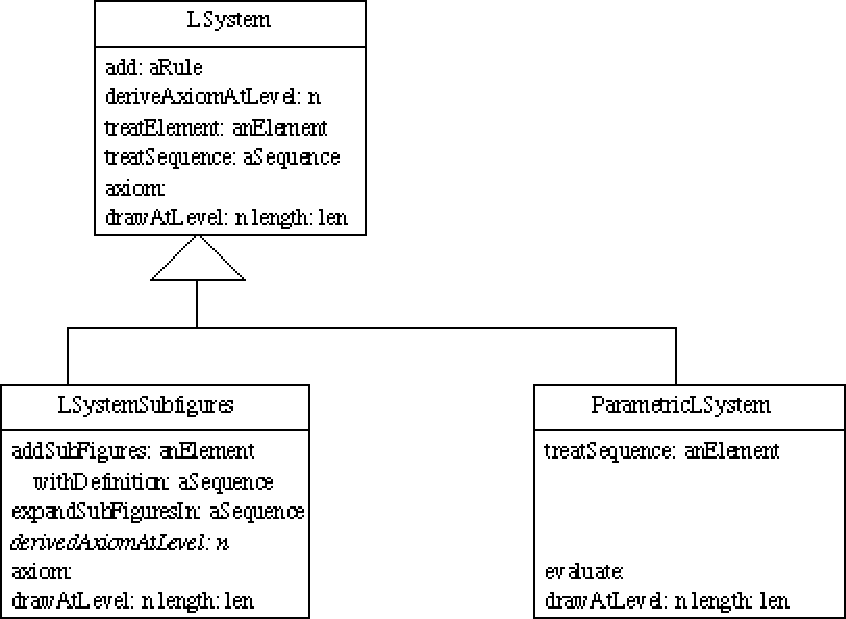
\includegraphics[width=10cm]{parametricinh}}
\caption{Relationships between the different classes participating in the LSystem application.}
\label{fig:parametric}
\end{figure}


Let us start by looking how we can evaluate the expression of a
fragment.  In the category \ct{'computing'}, define the method
\ct{evaluate:} that given a fragment composed by a symbol and an
expression, e.g., 2 * 3, returns a new fragment with the same symbol
and the value of the expression, e.g., 6. The following script 
shows some examples.

\begin{scriptwithtitle}{Illustration of \ct{evaluate:}}
| lsys |
lsys := ParametricLSystem new.
lsys evaluate: #(A 2 * 3) 
\emph{returns #(#A 6)}
lsys evaluate: #(A 2 - 3) 
\emph{returns #(#A -1)}
lsys evaluate: #(A 2 + 3)
\emph{returns  #(#A 5)}
\end{scriptwithtitle}

\paragraph{Hints.} There are several ways to implement the method 
\ct{evaluate:}. One interesting one is to use one of the method \ct{perform} defined on the class \ct{Object}.
For binary messages, \ct{perform:with:} allows one to say to an object
to execute the method whose selector is given with argument the second
argument.

\begin{scriptwithtitle}{Illustration of \ct{perform:with: use}}
2 perform: #* with: 3
\emph{returns 6}
\end{scriptwithtitle}

\hidden{
\begin{method}
ParametricLSystem>>evaluate: aFragment
   "self new evaluate: #(A 2 * 3) -> #(#A 6)"
   "self new evaluate: #(A 2 - 3) -> #(#A -1)"
   "self new evaluate: #(A 2 + 3) -> #(#A 5)"

   | op1 op2 oper |
   op1 := anElement second.
   oper := anElement third.
   op2 := anElement fourth.
   ^ Array with: anElement first with: (op1 perform: oper with: op2)
\end{method}
}


\begin{exonofig}
Enhance the method \ct{evaluate:} so that expressions evaluated can be
nested.  You can set as constraint that nested expression should
always be binary operations, that they should not contain symbols like
A or F and that they should always be between parenthesis.  For
example, (A 2 * (3 * 4)) should return (A 24), (A d * (3 * 4)) should
return (A d * 12)
\end{exonofig}

The next method we need is a method that given a sequence of elements
(fragment or symbols), a symbol representing a fragment argument and a
its value returns a new sequence where all the occurences of this
symbol have been replaced by its value and where evaluable expressions
are replaced by their values. Let us call this method
\ct{substitute:by:in:}. The following script shows some examples of
\ct{substitute:by:in:} use.

\begin{scriptwithtitle}{Illustration of \ct{substitute:by:in:}}
| lsys |
lsys := ParametricLSystem new.
lsys substitute: #d by: 1 in: #((A d) d)
\emph{returns #(#(#A 1) 1)}
lsys substitute: #d by: 1 in: #((A d * 2) d) 
\emph{returns  #(#(#A 2) 1)}
lsys substitute: #d by: 1 in: #((A d) (A 0) (A 1 * 3) d) 
\emph{returns #(#(#A 1) #(#A 0) #(#A 3) 1)}
\end{scriptwithtitle}

To implement \ct{substitute:by:in:} we need some helper methods: First
we need to implement a method that returns true if an element of a rule is
a fragment, false otherwise (Hint: you can check if the class of the object
passed as argument in from the class Array).

\begin{scriptwithtitle}{Illustration of \ct{isFragment:}}
| lsys |
lsys := ParametricLSystem new.
lsys isFragment: #(A d)
\emph{returns true}
lsys isFragment: #(A d * 3)
\emph{returns true}
lsys isFragment: #[
\emph{returns false}
lsys isFragment: #d
\emph{returns false}
\end{scriptwithtitle}


Second, we need to have a method that returns \ct{true} if a fragment
can be evaluated, i.e., with our current implementation this means
that the fragment is constitued by a symbol and an expression of the
form $number operation number$ as shown by the following scripts.

\begin{scriptwithouttitle}
| lsys |
lsys := ParametricLSystem new.
lsys shouldBeEvaluated: #(#A 2 #* 3)
\emph{returns true}
lsys shouldBeEvaluated: #(#A #d #* 3)
\emph{returns false}
\end{scriptwithouttitle}

Once we have the two helper methods defined the method
\ct{substitute:by:in:} can be implemented the following way. We
iterate over the collection of production elements. For each element
we check if this is a fragment. If this is not a fragment we simply
check if this is not the element that we want to substitute. If this
is the case we just return the value else the element because it does
not have to be changed. In case the element is a fragment we
substitute all the elements inside the fragment itself and check
wether the resulting fragment can be evaluated. If this is possible we
evaluate it else we just returning the new fragment whose symbols have
been subsituted.

\begin{method}
substitute: element by: value in: aCollection
                
   ^ aCollection 
        collect: [:each | 
                    (self isFragment: each) 
                       ifTrue: [|res|
                                res := self substitute: element 
                                            by: value 
                                            in: each.
                                (self shouldBeEvaluated: res) 
                                   ifTrue: [self evaluate: res]
                                   ifFalse: [res]]
                       ifFalse: [each = element
                                  ifTrue: [value]
                                  ifFalse: [each]]]
\end{method}


\subsection{Reconsidering String as Collections of Characters}\label{sec:stringascol}
In Chapter~\ref{ch:lsystem2} we chose to represent a rule as two
strings one for the left part and one for the right part. Some of you
may have wonder why we did not use a character for the left part.  Now
it is time to explain this choice! We made this choice because we knew
that for parametric L-Systems we would have a composed structure, like
an array or a collection, for the left part and not a single element.
As a string is a collection of characters if we were able to implement
something with strings we could reuse the methods for Parametric
L-Systems.

To illustrate this point, redefine the method \ct{treatSequence:} of
the class \ct{LSystem} as follow and check that all your previous
L-Systems still work:

\begin{method}
LSystem>>treatSequence: aCollection
   "Apply the rules to each element and return a string that 
   represents the result"
   
   | col |
   col := OrderedCollection new.
   aCollection
      do: [:anElement | col addAll: (self treatElement: anElement)].
   ^ col
\end{method}

This method creates an empty collection, an ordered collection, then
iterates over the collection of elements passed in argument: each
element is treated (by invoking the method \ct{treatElement:}) and the
returned result is added into the first created collection which is
finally returned.  What is important to see is that the method
\ct{treatElement:} may return a right part of a rule, so it returns a
collection of elements as shown by the following
\scriptref{src:treatel}.


\begin{scriptwithtitle}{Illustrating \ct{treatElement:}}\label{src:treatel}
| lsys rule1 |
lsys := ParametricLSystem new.
lsys axiom: '(A 100)'.
lsys angle: 88.
rule1 := ParametricLSRule 
             leftPart: '(A d)' 
             rightPart: '(F d)[+(A d / 1.456)][-(A d / 1.456)]'.
lsys add: rule1.
lsys treatElement: #+
\emph{returns #(#+)}.
lsys treatElement: #(#F 2)
\emph{returns #(#(#F 2))}.
lsys treatElement: #(#A 2)
\emph{returns #(#(#F 2) #[ #+ #(#A 1.373626373626374) #] #[ #- #(#A 1.373626373626374) #])}
\end{scriptwithtitle}

As show the following \scriptref{src:treatseq}, the method \ct{treatSequence:} should return a collection of fragments and symbols and not a collection of collection of fragments and symbols

\begin{scriptwithtitle}{Illustration of \ct{treatSequence:}.}\label{src:treatseq}
lsys treatSequence: #(#+).
\emph{returns anOrderedCollection(#+)}
self treatSequence: #((#F 2)).
\emph{returns an OrderedCollection(#(#F 2))}
lsys treatSequence: #(#+ #[ #(#F 2)).
\emph{anOrderedCollection(#+ #[ #(#F 2) #+)}
lsys treatSequence: #(#+ #(#A 2) #-)).
\emph{anOrderedCollection(#+ #(#F 2) #[ #+ #(#A 1.373626373626374) #] #[ #- #(#A 1.373626373626374) #] #-)}
\end{scriptwithtitle}

What is really interesting with this method \ct{treatSequence} defined
on class \ct{LSystem} is that it works for simple L-Systems but also
for Parametric L-Systems. This is due of the fact that a string is a
collection containing characters, \ct{String} is a subclass of
\ct{Collection}.  So any message sent to a collection are acceptable
by a string. In fact, we modified LSystem implementation after
discovering that pLSystem implementation could reuse it.

\subsection{The Last Methods and You are Done!}
Now the final method that is missing is the method
\ct{treatElement:}. This method is in fact doing the most important
work. Given an element of the production sequence it checks whether
this element match the current rules defined in the L-System,
evaluates the expressions contained in the using the argument values
and return the production of the L-System. Define the method \ct{treatElement:}
and if you fail read the following. 

The method \ct{treatElement:} should always returns a collection to satisfy the
\ct{addAll:} method used on its result in the method
\ct{treatSequence} presented above.
So the method \ct{treatSequence:} checks whether the passed element is
a fragment, if this is not the case, this means that the element is a
symbol such as \ct{[}, \ct{+} so such a symbol is put inside an array
and the method exits.  When the element is a fragment, the method
checks whether there is rule matching this element. If there is no
rule then a collection having as single element the fragment is
return. This is again done because we want to have a fragment inside
the production rule and returning simply a fragment would not work
because \ct{addAll:} would add not a fragment but all its elements
into the resulting sequence. If the fragment matches a rule, the
method then returns the right part of the matched rule where all the
symbol have been replaced by

In~\scriptref{src:treatel}, for example the fragment $(A 2)$ matches
the rule $(A d) \rightarrow (F d)[+(A d / 1.456)][-(A d / 1.456)]$
therefore the result is to substitute $d$ by 2 in the right part, to
evaluate the expressions that can be evaluate and return the new
sequence of elements. Here the result is then $(F 2) [+(A 1.373626373626374)][-(A 1.373626373626374)]$

\begin{method}
treatElement: anElement 
   "returns an array containing an Element if anElement is a single symbol
   or if anElement is not a left part of a rule, else returns an array representing the    
   right part of a rule. Note that if this is a fragment it is evaluated"
        
   | selectedRule |
   (self isFragment:anElement) 
          ifFalse: [^ Array with: anElement].

   selectedRule := rules detect: [:each | each doesMatch: anElement]
                         ifNone: [nil].
   ^selectedRule isNil 
       ifTrue: [Array with: anElement]
       ifFalse: [self substitute: (selectedRule leftPart second)                        
                      by: (anElement second)  
                      in: selectedRule rightPart]
\end{method}

\paragraph{A Powerful Turtle}
Now the only thing that we have to do is to change the way the turtle
interpret the information we give it. Indeed the turtle now has to
know how to interpret elements (composed fragments with values and
simple symbols). We give you the following code, so that you can test
faster your implementation and have fun.  The method
\ct{interpretExpression: anExpression angle: degree magnified: times}
interprets a single element.

\begin{method}
TurtleWithMemory>>interpretExpression: anExpression angle: degree magnified: times 
   | aCharacter |
   (anExpression isKindOf: Array)
      ifTrue: [aCharacter := anExpression first]
      ifFalse: [aCharacter := anExpression].
   aCharacter = #F
      ifTrue: [self go: anExpression second * times]
      ifFalse: [aCharacter = #+
	          ifTrue: [self turnLeft: degree]
                  ifFalse: [aCharacter = #-
                                ifTrue: [self turnRight: degree]
                                ifFalse: [aCharacter = #[
                                              ifTrue: [self pushCurrentState]
                                              ifFalse: [aCharacter = #] 
                                                          ifTrue: [self restoreState]]]]]
\end{method}

\begin{method}
TurtleWithMemory>>interpretExpression: aString angle: degree 
   self
      interpretExpression: aString
      angle: degree
      magnified: 1
\end{method}

Define the methods \ct{interpretExpressions: aCollection angle: degree
magnified: times} and \ct{interpretExpressions: aCollection angle:
degree} that invokes the previously defined methods on collection of
elements.



If you want to automate the sending of production results to a turtle,
use the following method, or create your own. With such a method you
can now ask a pL-System to derive itself a number of times and to draw
itself.

\begin{method}
ParametricLSystem>>drawAtLevel: n magnified: times 
   | turtle derivation |
   turtle := TurtleWithMemory new.
   derivation := self deriveAxiomAtLevel: n.
   turtle
      interpretExpressions: derivation
      angle: angle
      magnified: times.
    ^ derivation
\end{method}




\section{Fun with pL-Systems}
Now we present you some interesting pL-Systems and discuss some
differences in modelling.



\begin{tabbing}
\=aaa\=aaa\=aaa\=aaaaaaaaa\=aaaaaaaaa\=aaaaaaaaa\=aaaaaaaaa\=aaaaaaaaa\=aaaaaaaaa\kill
Cactus (Figure~\ref{fig:p47})\\
\>\>\>\> \emph{Axiom} \>\>\emph{A(200)}\\
\>\>\>\> \emph{Angle} \>\>81 degree\\
\>\>\>\> \emph{Rule}  \>\>\emph{F(x) $\rightarrow$ F(x * 0.3) + F(x * 0.4582)- - F(x*0.4582) + F(x*0.7)}
\end{tabbing}

The values of the Cactus pL-System come from the fact that this
L-System is based on the idea of filling a square triangle. The expression we gave is based on the following one 
\emph{F(x)$\rightarrow$ F(x*p)+F(x*h)--F(x*h)+F(x*q)} where $p+q = hypotenuse$, $p$ is the distance on the hypotenuse from one corner to the height of the triangle, $q$ is the other  distance on the hypotenuse from the other corner to the height of the triangle, $h$ is the height of the rectangle issued from the square angle. So if $c$ is the hypotenuse length, $p=0.3$, $q=0.7$ and $h = \sqrt{p*q}$.


\begin{figure}[!htbp]
\centerline{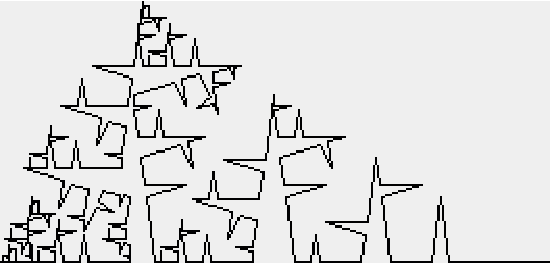
\includegraphics{p47}}
\caption{Leaf 2, Level = 5,}
\label{fig:p47}
\end{figure}



\begin{tabbing}
\=aaa\=aaa\=aaa\=aaaaaaaaa\=aaaaaaaaa\=aaaaaaaaa\=aaaaaaaaa\=aaaaaaaaa\=aaaaaaaaa\kill
Leaf 2 (Figure~\ref{fig:plant180})\\
\>\>\>\> \emph{Axiom} \>\>\emph{A(0)}\\
\>\>\>\> \emph{Angle} \>\>45 degree\\
\>\>\>\> \emph{Rule}  \>\>\emph{A(d) $\rightarrow$ F(2)[+A(0)][-A(0)]F(2)A(0)}\\
\>\>\>\> \emph{Rule}  \>\>\emph{F(d) $\rightarrow$ F(d * 1.456)}
\end{tabbing}

\begin{figure}[!htbp]
\centerline{\includegraphics{plant180}}
\caption{Leaf 2, Level = 8, Magnified 1.2}
\label{fig:plant180}
\end{figure}



L-Systems can create forms by appending segments of decreasing length
to the structures obtained in previous derivation steps like the
following pL-System T Growing 1 does.  Once a segment is treated, its
length does not change as shown by the top figure of the
Figure~\ref{fig:Tgrow1}.

\begin{tabbing}
\=aaa\=aaa\=aaa\=aaaaaaaaa\=aaaaaaaaa\=aaaaaaaaa\=aaaaaaaaa\=aaaaaaaaa\=aaaaaaaaa\kill
T 1 (Figure~\ref{fig:TGrow1})\\
\>\>\>\> \emph{Axiom} \>\>\emph{A(1)}\\
\>\>\>\> \emph{Angle} \>\>88 degree\\
\>\>\>\> \emph{Rule}  \>\>\emph{A(s) $\rightarrow$ F(s)[+A(s/1.456)][-A(s/1.456)]}\\
\end{tabbing}

A structure with identical proportions can be obtained by appending
segments of constant length and increasing the lengths of the
previously created segments by a constant as shown by the bottom
figure in Figure~\ref{fig:TGrow1}.

\begin{tabbing}
\=aaa\=aaa\=aaa\=aaaaaaaaa\=aaaaaaaaa\=aaaaaaaaa\=aaaaaaaaa\=aaaaaaaaa\=aaaaaaaaa\kill
T 2(Figure~\ref{fig:TGrow2}\\
\>\>\>\> \emph{Axiom} \>\>\emph{A(0)}\\
\>\>\>\> \emph{Angle} \>\>88 degree\\
\>\>\>\> \emph{Rule}  \>\>\emph{A(d) $\rightarrow$ F(1)[+A(0)][-A(0)]}\\
\>\>\>\> \emph{Rule}  \>\>\emph{F(d) $\rightarrow$ F(d * 1.456)}
\end{tabbing}

\begin{figure}[!htbp]
\centerline{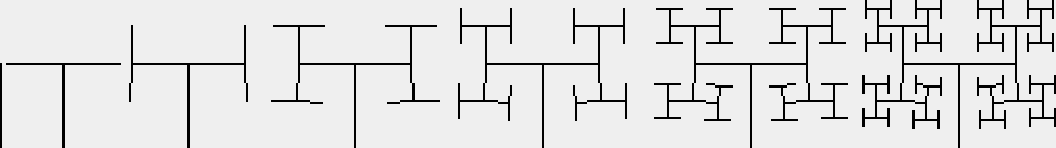
\includegraphics[width=10cm]{TGrow2}}
\centerline{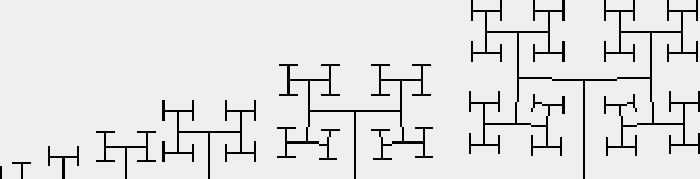
\includegraphics[width=10cm]{TGrow1}}
\caption{Two different ways of creating figures. The top figure is created by appending segments of decreasing lengths. The bottom figure is created by increasing the length of previouslycreated segments.}
\label{fig:TGrow1}
\end{figure}


















\section{Models of Compound Leaves}

\cite{prus90a} shows how pL-Systems can model compound leaves. 
He introduces the following pL-Systems, one representing symmetrical
branches and the other one producing alternate branches. $D$
represents the apical delay, i.e., the time needed to branch and $R$
the internode elongation rate. These two values are constants that can
be changed to produce different leaves. Try the values proposed in the
tables~\ref{tab:sym} and \ref{tab:asym} extracted from \cite{prus90a}.
Pay attention that some of the results have to be minimized or
maximized using the method \ct{drawAtLevel:magnified:} and that the
parameters may have to be changed.

\begin{figure}[!htbp]
\centerline{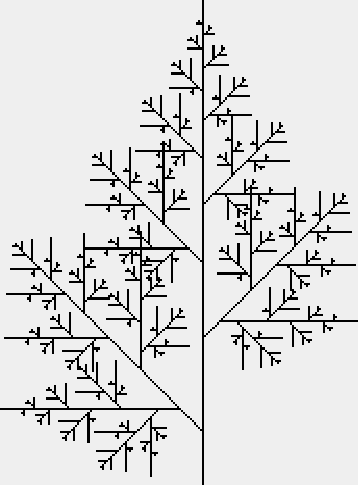
\includegraphics{alternate130}}
\caption{}
\label{fig:alternate}
\end{figure}


\begin{tabbing}
\=aaa\=aaa\=aaa\=aaaaaaaaa\=aaaaaaaaa\=aaaaaaaaa\=aaaaaaaaa\=aaaaaaaaa\=aaaaaaaaa\kill
Symmetrical Compound Leave (Figure~\ref{fig:plant180})\\
\>\>\> \emph{Axiom} \>\>\emph{A(0)}\\
\>\>\> \emph{Angle} \>\>45 degree\\
\>\>\> \emph{Rule}  \>\>\emph{A(d): d > 0 $\rightarrow$ A(d - 1)}\\
\>\>\> \emph{Rule}  \>\>\emph{A(d): d = 0 $\rightarrow$ F(1)[+A(D)][-A(D)]F(1)A(0)}\\
\>\>\> \emph{Rule}  \>\>\emph{F(a): -- $\rightarrow$ F(a * R)}
\end{tabbing}

\begin{table}
\begin{center}
\begin{tabular}{|c|c|c|}\hline 
\textbf{D} &\textbf{R}& \textbf{Derivation level}\\ \hline
0& 2.00& 10\\ \hline 
1& 1.50& 16\\ \hline
2& 1.36& 21\\ \hline 
4& 1.23& 30\\ \hline 
\end{tabular}
\end{center}
\caption{Some  D and R values for the symmetrical model.}\label{tab:sym}
\end{table}


\begin{tabbing}
\=aaa\=aaa\=aaa\=aaaaaaaaa\=aaaaaaaaa\=aaaaaaaaa\=aaaaaaaaa\=aaaaaaaaa\=aaaaaaaaa\kill
Alternate Branching Plant (Figure~\ref{fig:alternate130})\\
\>\>\> \emph{Axiom} \>\>\emph{A(0)}\\
\>\>\> \emph{Angle} \>\>45 degree\\
\>\>\> \emph{Rule}  \>\>\emph{A(d): d > 0 $\rightarrow$ A(d - 1)}\\
\>\>\> \emph{Rule}  \>\>\emph{A(d): d = 0 $\rightarrow$ F(1)[+A(D)]F(1)B(0)}\\
\>\>\> \emph{Rule}  \>\>\emph{B(d): d > 0 $\rightarrow$ B(d - 1)}\\
\>\>\> \emph{Rule}  \>\>\emph{B(d): d = 0 $\rightarrow$ F(1)[-B(D)]F(1)B(0)}\\
\>\>\> \emph{Rule}  \>\>\emph{F(a): -- $\rightarrow$ F(a * R)}
\end{tabbing}

\begin{table}
\begin{center}
\begin{tabular}{|c|c|c|}\hline 
\textbf{D} &\textbf{R}& \textbf{Derivation level}\\ \hline
1& 1.36& 20\\ \hline
4& 1.18& 34\\ \hline
\end{tabular}
\end{center}
\caption{Some  D and R values for the symmetrical model.}\label{tab:asym}
\end{table}


Try to produce your own pL-Systems, for example, you can modify the delay
of the rule selection by changing the value of the argument passed. 







\section{Enhancements}


\begin{itemize}
\item Rule printing
\item ensuring that the right class is used for rules. 

\item Introduce a way to manage constants:
For example using collection of pairs and substituting the value
before the rewritting.  

\item The computation of the value can be radically speed up by caching the results and checking if they have not already been computed before computing them. This is especially relevant in our case where the  computation uses always the same number. 

\item introduce the possibility to handle multiple parameters



 
\end{itemize}

\begin{exonofig}
Use parametric L-System  in the L-Systems modeling plant. You can for example
control in a finer manner how the branches should grow.
\end{exonofig}



\ifx\wholebook\relax\else\end{document}\fi
